\begin{figure*}[t]
    \centering
    \setlength{\resLenTwo}{2in}
    \setlength{\resLen}{.1\textwidth}
    \addtolength{\tabcolsep}{-3pt}
    \small
    \begin{tabular}{ccc|ccc|ccc}
        \multicolumn{3}{c|}{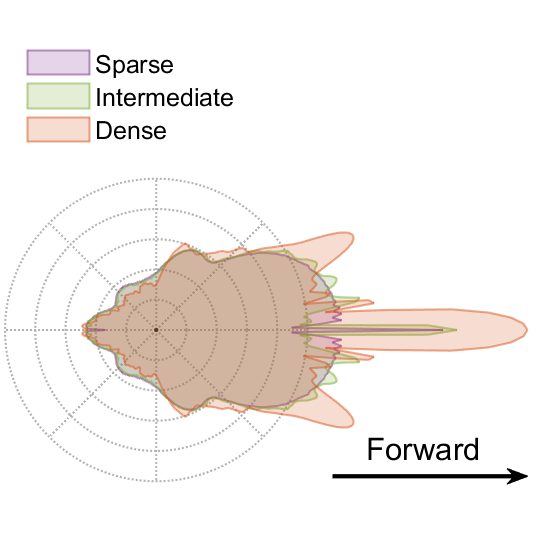
\includegraphics[width=3.\resLen]{pfunc/distance.png}} &
        \multicolumn{3}{c|}{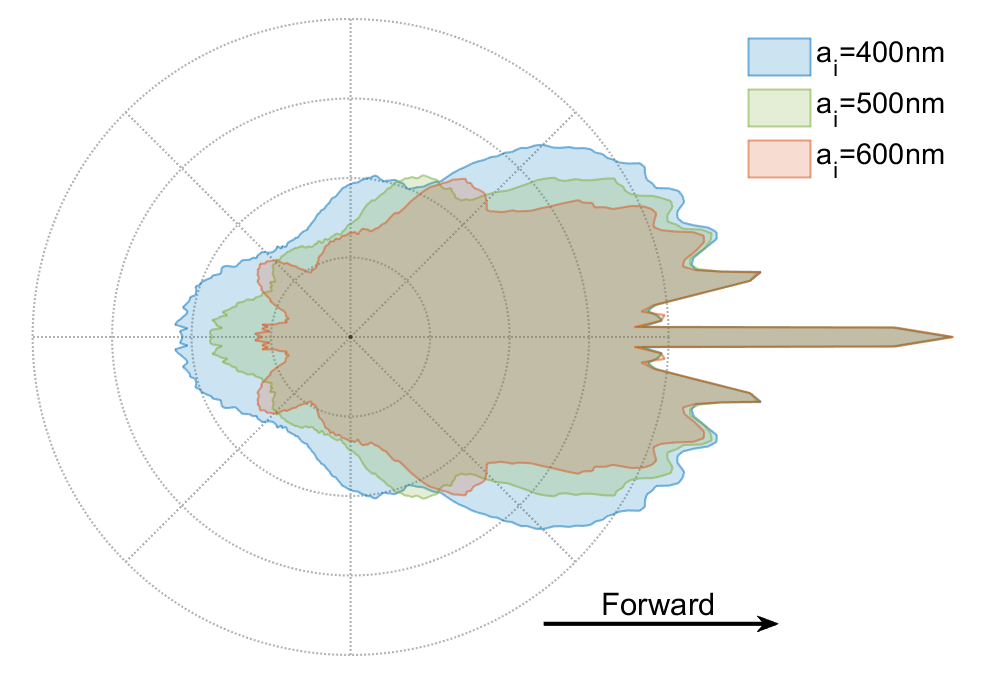
\includegraphics[width=3.\resLen]{pfunc/radius.png}} &
        \multicolumn{3}{c}{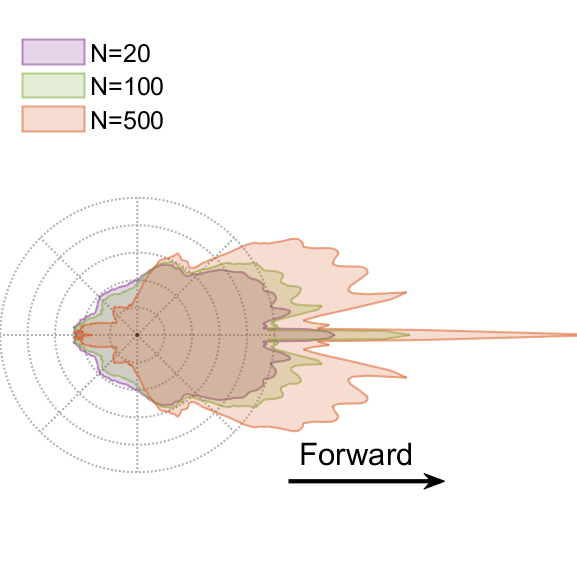
\includegraphics[width=3.\resLen]{pfunc/number.png}} \\[-5pt]
        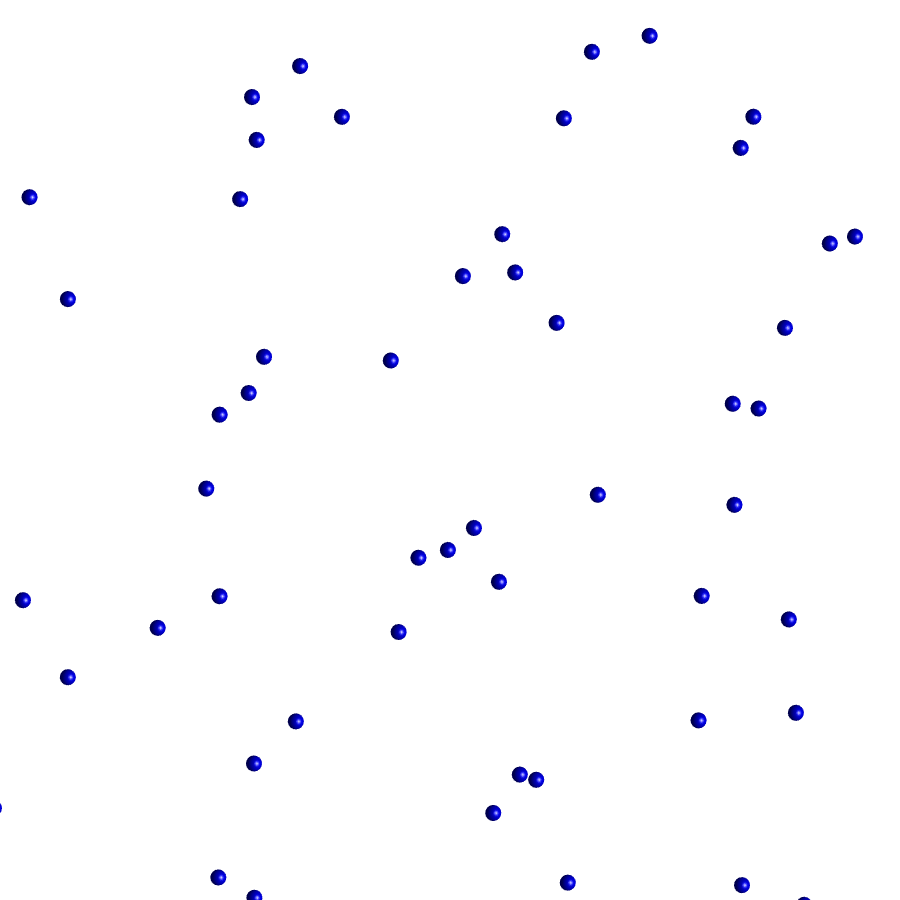
\includegraphics[width=\resLen]{particle/validate2_D1_N100_500nm.png} &
        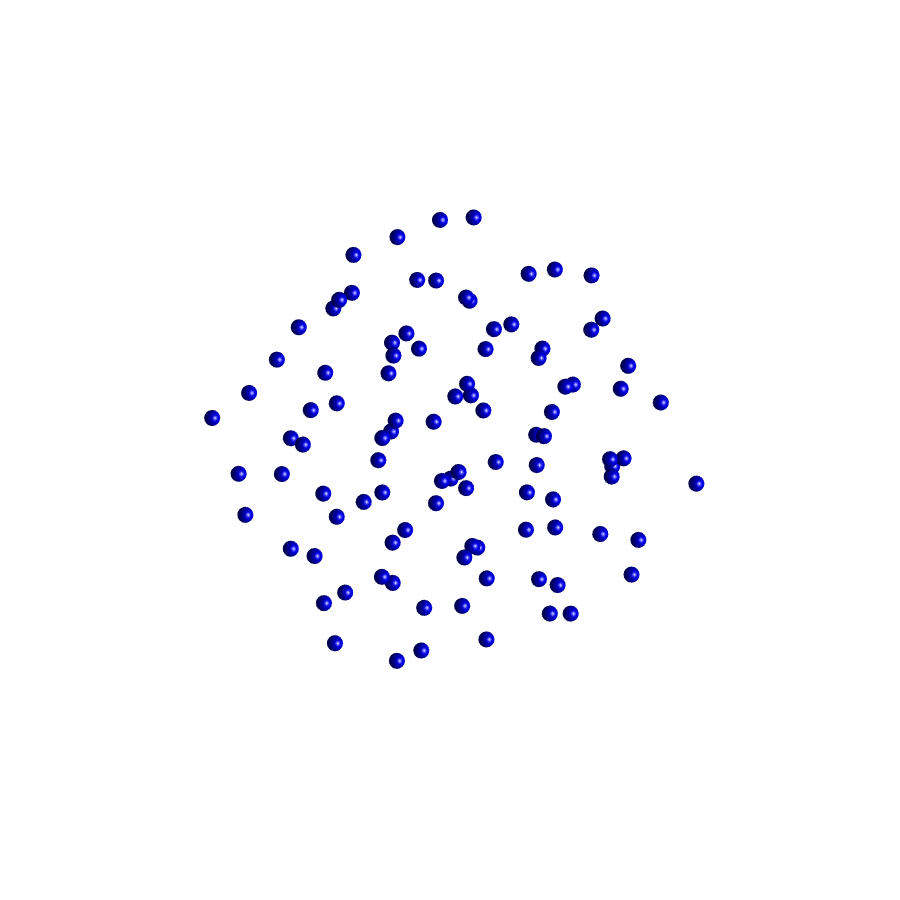
\includegraphics[width=\resLen]{particle/validate3_D2_N100_500nm.png} &
        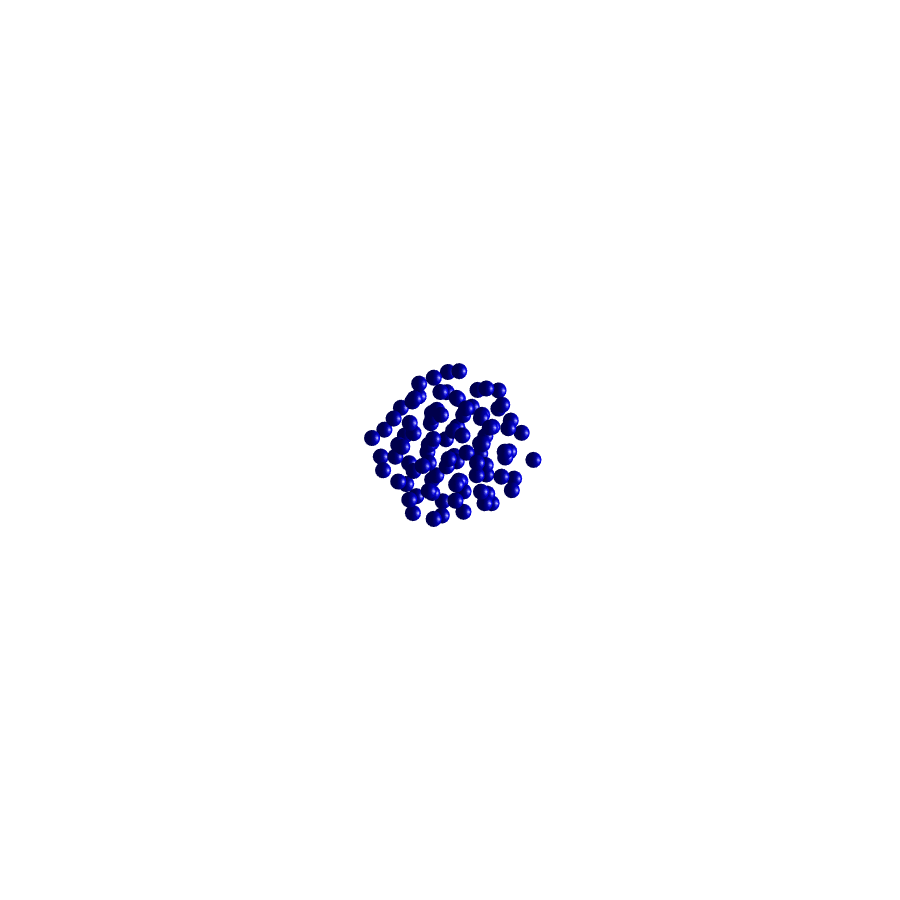
\includegraphics[width=\resLen]{particle/validate4_D3_N100_500nm.png} &
        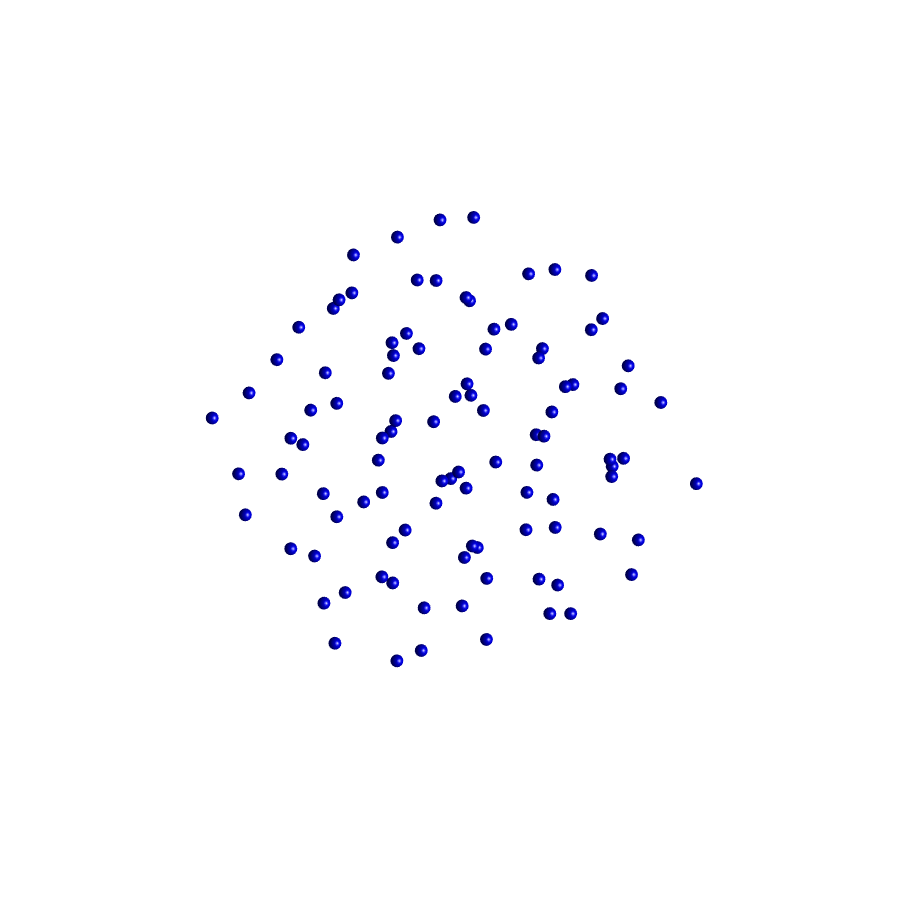
\includegraphics[width=\resLen]{particle/validate5_D2_N100_400nm.png} &
        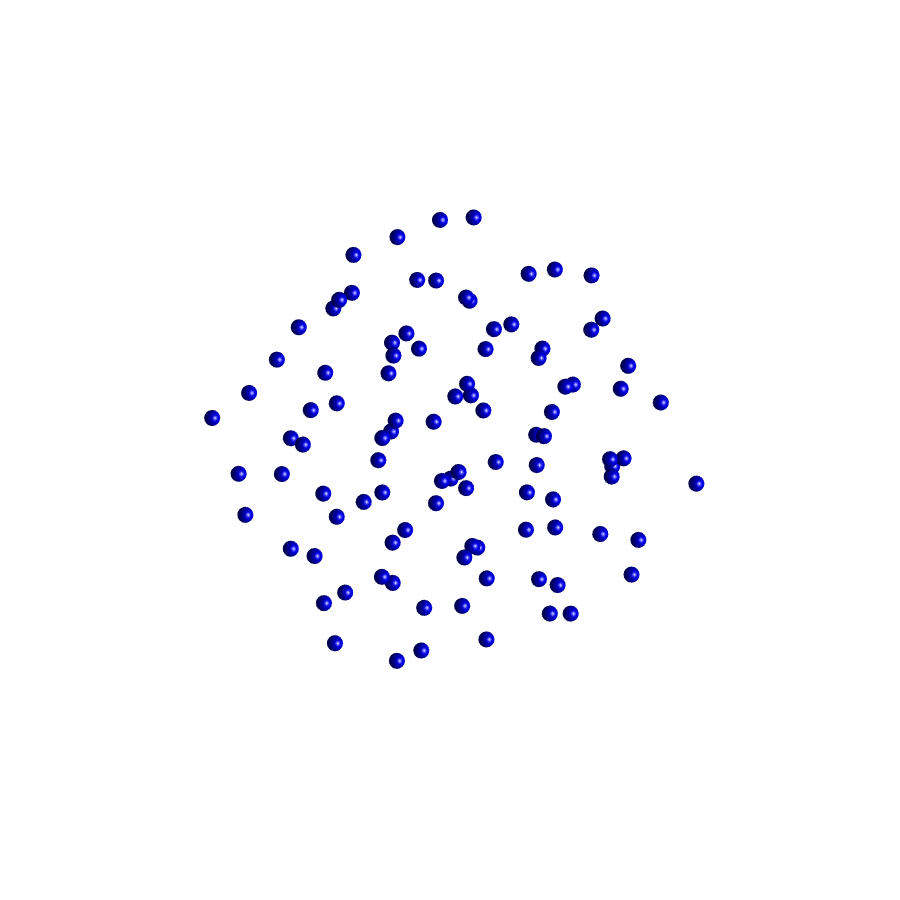
\includegraphics[width=\resLen]{particle/validate3_D2_N100_500nm.png} &
        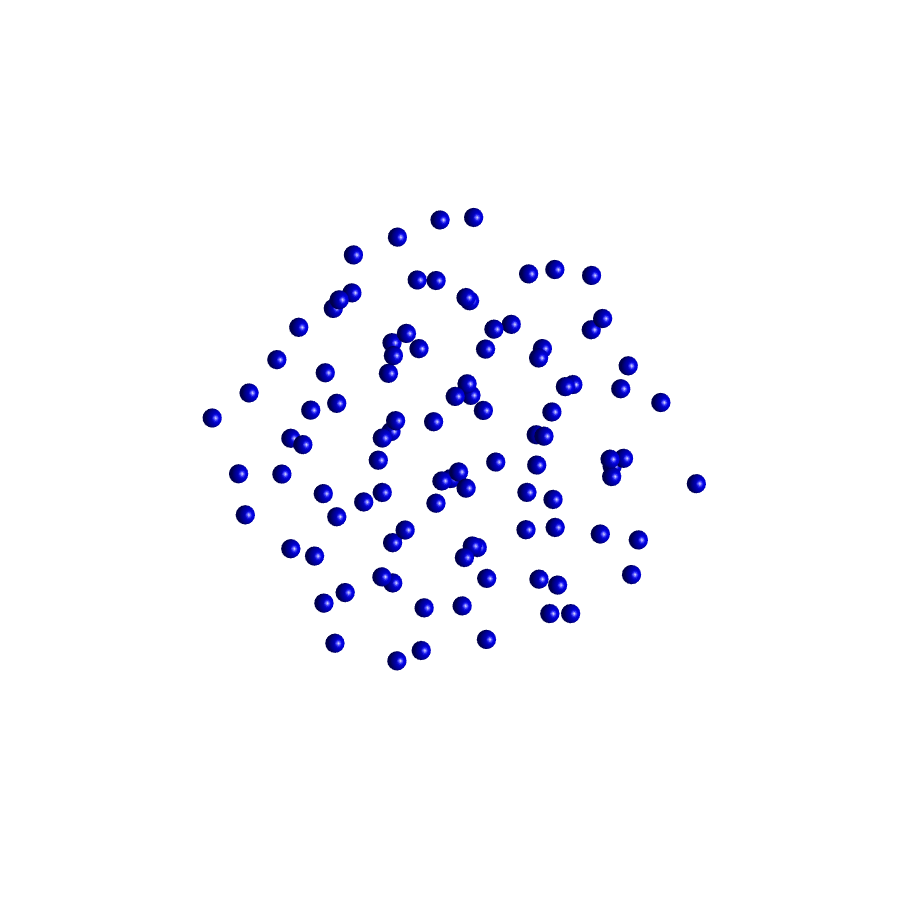
\includegraphics[width=\resLen]{particle/validate7_D2_N100_600nm.png} &
        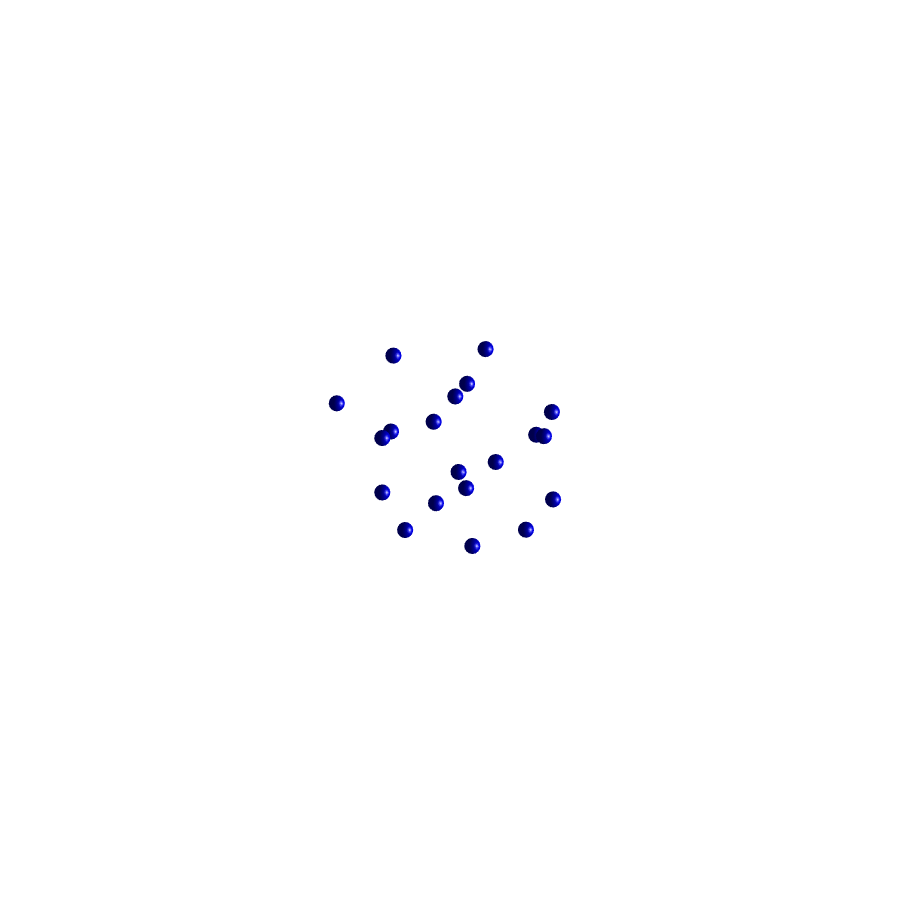
\includegraphics[width=\resLen]{particle/validate8_D2_N20_500nm.png} &
        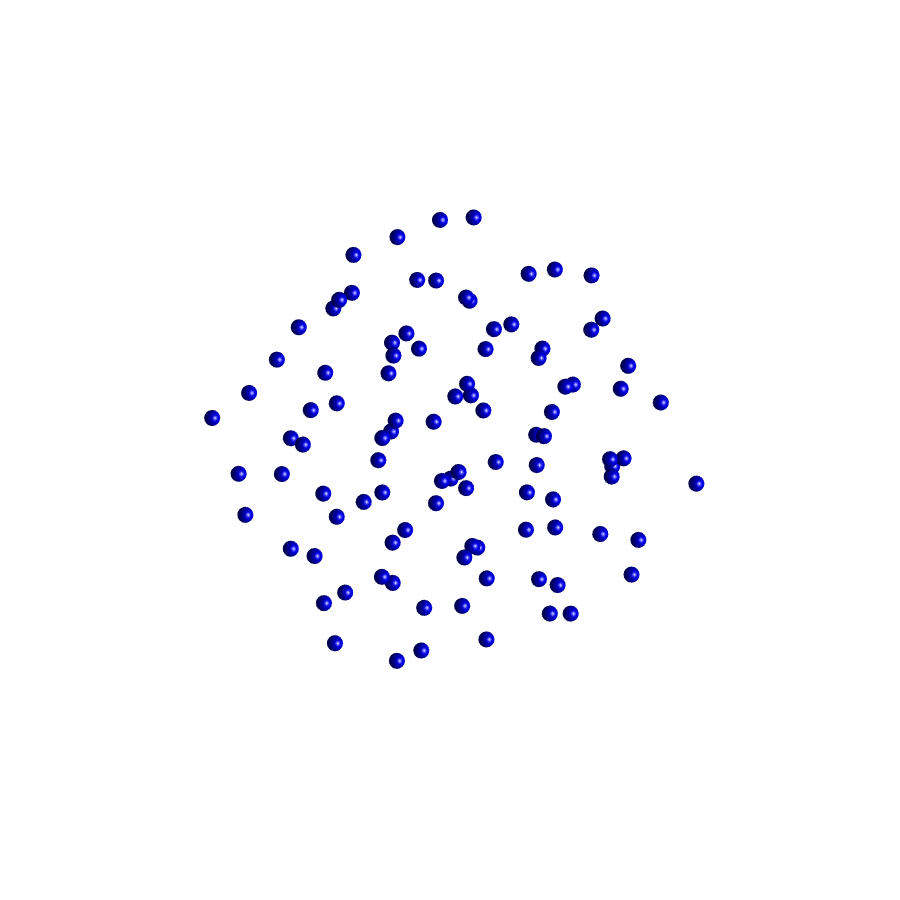
\includegraphics[width=\resLen]{particle/validate3_D2_N100_500nm.png} &
        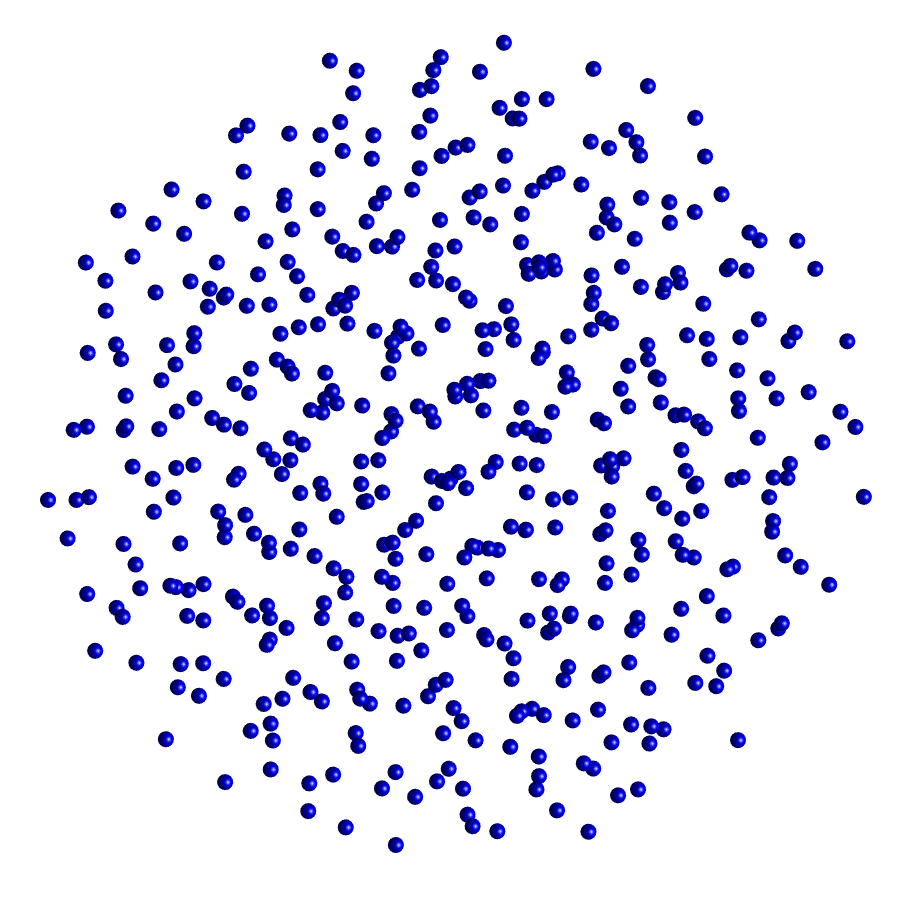
\includegraphics[width=\resLen]{particle/validate10_D2_N500_500nm.png} 
        \\
        Sparse & Intermediate & Dense & $\radius_i$=400nm & $\radius_i$=500nm & $\radius_i$=600nm &
        $\Ncls=20$ & $\Ncls=100$ & $\Ncls=500$ \\[5pt]
        \multicolumn{3}{c}{\bfseries (a) Varying particle spacing} &
        \multicolumn{3}{c}{\bfseries (b) Varying particle radii} &
        \multicolumn{3}{c}{\bfseries (c) Varying particle counts}
    \end{tabular}
    \caption{\label{fig:ablation}
        Comparison of the resulting \rev{(normalized)} phase function for different cluster parameters, for a planar incident field at $\lambda=700$nm. Unless mentioned otherwise, the clusters have $\Ncls=100$ particles, and each particle has radius $\radius_i=500$nm. For each phase function, we vary: (a) The distance between particles within the cluster; (b) The particle size $\radius_i$; and (c) The number of particles $\Ncls$.
        \rev{We visualize all phase functions in logarithmic scale to better show their low-magnitude regions.}
    }
\end{figure*}